\documentclass[10pt]{beamer}

%%%
% PREAMBLE FOR THIS DOC 
%%%
%https://tex.stackexchange.com/questions/68821/is-it-possible-to-create-a-latex-preamble-header
\usepackage{/Users/miw267/Repos/csci246_spring2025/slides/preambles/beamer_preamble_for_CSCI246}


%%% TRY TO RESHOW TOC AT EACH SECTION START (with current section highlighted)
% Reference: https://tex.stackexchange.com/questions/280436/how-to-highlight-a-specific-section-in-beamer-toc
\newcommand\tocforsect[2]{%
  \begingroup
  \edef\safesection{\thesection}
  \setcounter{section}{#1}
  \tableofcontents[#2,currentsection]
  \setcounter{section}{\safesection}
  \endgroup
}


\usepackage[normalem]{ulem} % for strikeout (\sout)

%%%% HERES HOW TO DO IT CORRECTLY
% FIRST IN .STY FILE, DO
%\usetheme[sectionpage=none]{metropolis}
% THEN AT EACH SECTION DO
%\begin{frame}{Outline}
%  \tableofcontents[currentsection]	
%\end{frame}



%\setbeamertemplate{navigation symbols}{}
%\setbeamertemplate{footline}[frame number]{}


%%%
% DOCUMENT
%%%

\begin{document}

%\maketitle

%% Title page frame
%\begin{frame}
%    \titlepage 
%\end{frame}



\title{04/14/2025: Connection}
\author{CSCI 246: Discrete Structures}
\date{Textbook reference: Sec 49, Scheinerman}

\begin{frame}
    \titlepage 
\end{frame}


\begin{frame}
\small
%\begin{mygreenbox}[title=Graded Quiz Pickup]
%Quizzes are in the front of the room, grouped into four bins (A-G, H-L, M-R, S-Z) by last name. The quizzes are upside down with your last name on the back. Come find yours before, during, or after class. Only turn the quiz over if it's yours.
%\end{mygreenbox} 
%\vfill 
\begin{myredbox}[title=Problems Quiz On Wednesday]
 Hence, our final problems quiz will be on WEDNESDAY 04/16.  The topics that will be covered are:
\begin{itemize}
\item Fundamentals of Graph Theory (Scheinerman Sec 47; see group exercises and reading quiz from 04/09)
\item Subgraphs (Scheinerman Sec 48; see group exercises and reading quiz from 04/11) 
\item Connection (Scheinerman Sec 49; we will cover this today)
\end{itemize}
\end{myredbox}
\vfill 
\begin{myyellowbox}[title=Today's Agenda]
\begin{itemize}
	\item Reading quiz (5 mins)
	\item Review solutions to previous group exercises ($\approx$ 10 mins)
	\item New group exercises ($\approx$ 20 mins)
	\item Review solutions to new group exercises ($\approx$ 10 mins)
\end{itemize}


\end{myyellowbox}
\vfill 

\end{frame}






\begin{frame}[standout]
Feedback on Friday's Quizzes
\end{frame}


\begin{frame}{Reading Quiz Scores}
\small 
\begin{figure}[ht]
        \centering
        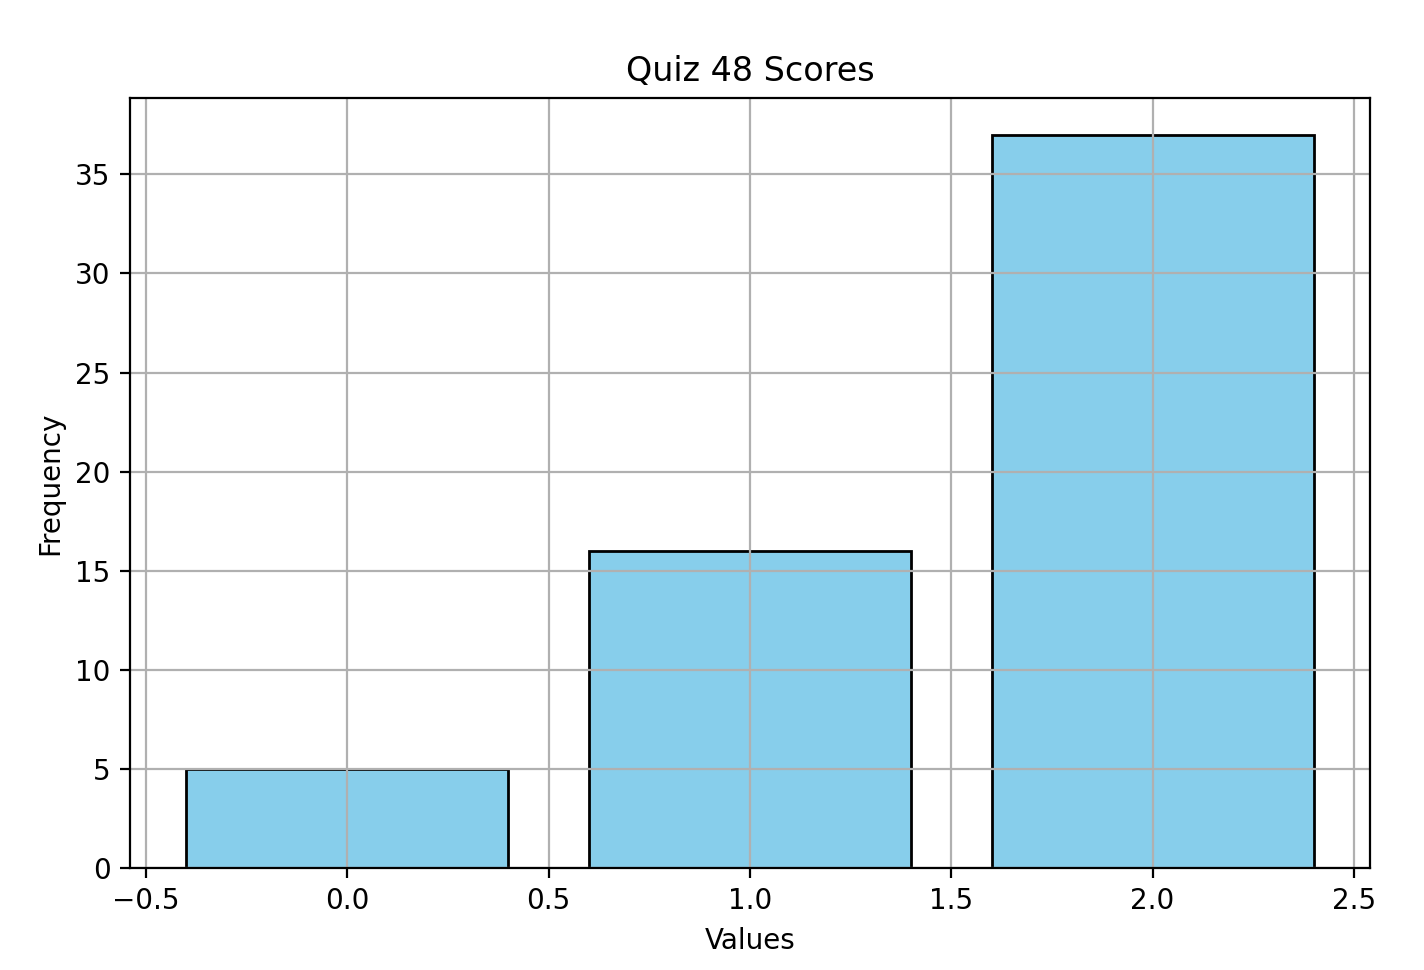
\includegraphics[width=.7\textwidth]{images/reading_quiz_scores}
   		 \caption{Median Score = 2/2 (100\%)}
\end{figure}
\vfill 
\textbf{Grading Rubric:}  
\begin{enumerate}
\item (1 point) Clique.
\item (1 point) Independent set.
\end{enumerate}







\end{frame}	


\begin{frame}{Problem Quiz Scores}
\footnotesize 
\begin{figure}[ht]
        \centering
        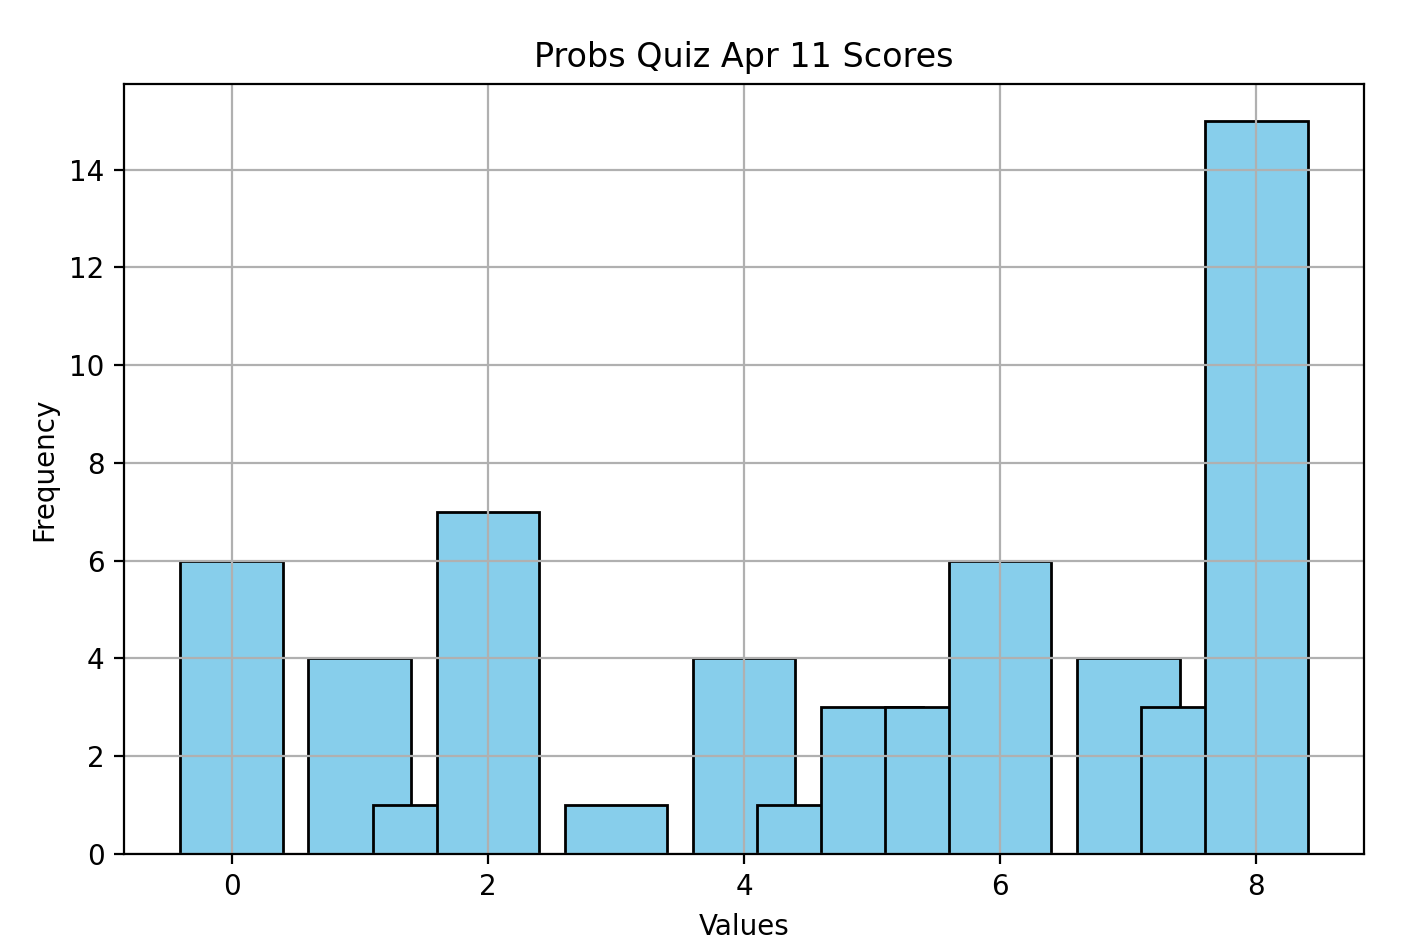
\includegraphics[width=.5\textwidth]{images/problem_quiz_scores}
   		 \caption{Median Score = 5/8 (68.75\%)}
\end{figure}
\vfill 
\textbf{Grading Rubric:}  
\begin{enumerate}
\item (4 points) 1 point for getting the roots correct, 1 point for choosing the correct form out of the two listed, 1 point for solving for $c_1, c_2$ correctly, 1 point for the final equation being stated correctly (given $c_1$ and $c_2$).
\item (4 points) If you appealed to the definitions:  2 points for correctly proving Big O, 2 points for correctly proving Big Omega.  Note, however, there is a shortcut solution, which is to simply reference the theorem on polynomial orders. That is also a perfectly acceptable answer worth 4 points.
\end{enumerate}



\end{frame}	


\begin{frame}[standout]
Today's quiz
\end{frame}

\begin{frame}
%\small 

\begin{mygreenbox}[title=\text{Reading quiz (Connection)}]

The argument below is from the text.  Is it right or wrong?  If it's wrong, what is the problem with it?
\end{mygreenbox}
\vfill 
\begin{myyellowbox}[title=\text{Reference passage from text}]
\begin{minipage}{.68\textwidth}
Is the is-connected-to relation transitive? Suppose, in a graph $G$, we know that $x$ is connected to $y$ and that $y$ is connected to $z$.  We want to prove that $x$ is connected to $z$. \\
\vspace{.15cm}

Since $x$ is connected to $y$, there must be an $(x,y)$-path; let's call it $P$.  And since $y$ is connected to $z$, there must be a $(y,z)$-path.  Let's call it $Q$.  Notice that the last vertex of $P$ is the same as the first vertex of $Q$ (it's y).  Therefore, we can form the concatenation $P+Q$, which is an $(x,z)$-path.  Therefore $x$ is connected to $z$.
\end{minipage} %
\hfill 
\begin{minipage}{.28\textwidth}
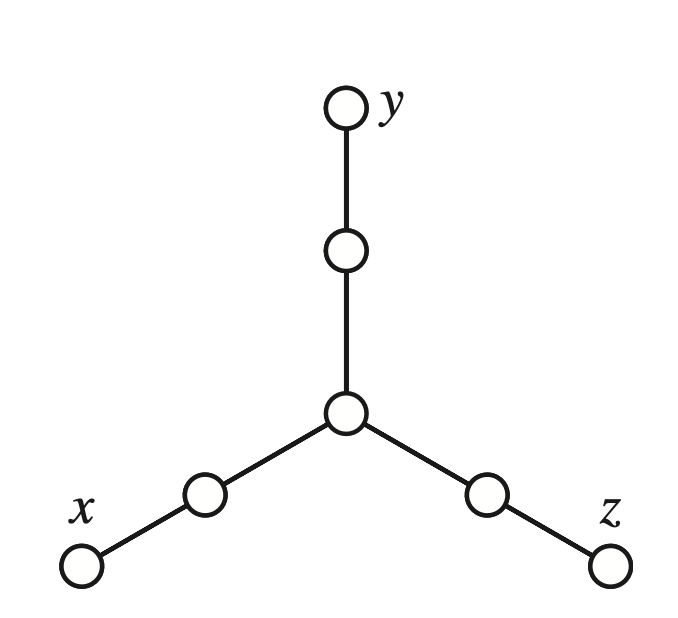
\includegraphics[width=\linewidth]{images/transitivity_of_connection.png}
\end{minipage}

\end{myyellowbox}

\end{frame}

\begin{frame}[standout]
Q\&A On Previous Group Exercises
\end{frame}


%\begin{frame}[standout]
%Thoughts On Connection
%\end{frame}

\begin{frame}[standout]
Group exercises
\end{frame}

\begin{frame}
\footnotesize 
\vfill 
\begin{columns}
\begin{column}{0.33\textwidth}
aaron.loomis: 13 \\ 
adam.wyszynski: 9 \\ 
alexander.knutson: 20 \\ 
anthony.mann: 15 \\ 
blake.leone: 14 \\ 
bridger.voss: 1 \\ 
caitlin.hermanson: 15 \\ 
cameron.wittrock: 4 \\ 
carsten.brooks: 17 \\ 
carver.wambold: 12 \\ 
colter.huber: 2 \\ 
conner.reed1: 1 \\ 
connor.mizner: 8 \\ 
connor.yetter: 16 \\ 
derek.price4: 8 \\ 
devon.maurer: 17 \\ 
emmeri.grooms: 18 \\ 
erik.moore3: 16 \\ 
ethan.johnson18: 16 \\ 
evan.barth: 6 \\ 
evan.schoening: 2 \\\end{column}
\begin{column}{0.33\textwidth}
griffin.short: 9 \\ 
jack.fry: 14 \\ 
jacob.ketola: 8 \\ 
jacob.shepherd1: 12 \\ 
jada.zorn: 2 \\ 
jakob.kominsky: 5 \\ 
james.brubaker: 3 \\ 
jeremiah.mackey: 15 \\ 
jett.girard: 10 \\ 
john.fotheringham: 3 \\ 
jonas.zeiler: 11 \\ 
joseph.mergenthaler: 6 \\ 
joseph.triem: 17 \\ 
julia.larsen: 18 \\ 
justice.mosso: 5 \\ 
kaden.price: 19 \\ 
lucas.jones6: 21 \\ 
luka.derry: 4 \\ 
luke.donaldson1: 7 \\\end{column}
\begin{column}{0.33\textwidth}
lynsey.read: 19 \\ 
mason.barnocky: 10 \\ 
matthew.nagel: 11 \\ 
micaylyn.parker: 14 \\ 
michael.oswald: 5 \\ 
nolan.scott1: 4 \\ 
owen.obrien: 13 \\ 
pendleton.johnston: 9 \\ 
peter.buckley1: 13 \\ 
reid.pickert: 19 \\ 
ryan.barrett2: 11 \\ 
samuel.hemmen: 1 \\ 
samuel.mosier: 7 \\ 
samuel.rollins: 6 \\ 
sarah.periolat: 20 \\ 
timothy.true: 10 \\ 
tristan.nogacki: 3 \\ 
tyler.broesel: 18 \\ 
william.elder1: 12 \\ 
yebin.wallace: 20 \\ 
zeke.baumann: 7 \\\end{column}
\end{columns}
\vfill
\end{frame}

\begin{frame}{Group exercises}
\small 
\noindent
\begin{minipage}{0.6\textwidth}
\begin{enumerate}
	\item  Let $G$ be the graph in the top figure.   (a) How many different paths are there from $a$ to $b$? (b) How many different walks are there from $a$ to $b$?
	\item Let $G$ be a graph.  A path $P$ in $G$ that contains all the vertices of $G$ is called a \textit{Hamiltonian Path}.  Prove that the graph in the bottom figure does not have a Hamiltonian path.
    \item How many Hamiltonian paths does a complete graph on $n \geq 2$ vertices have?
    \item Let $G$ be a graph with $n \geq 2$ vertices.  
    \begin{itemize}
    \item[a.] Prove that if G has at least $\binom{n-1}{2} +1$ edges, then $G$ is connected.
    \item[b.] Show that the result in (a) is best possible; that is, for each $n \geq 2$, prove there is a graph with 	$\binom{n-1}{2}$ edges that is not connected.
    \end{itemize}

\end{enumerate}
\end{minipage}%
\hfill
\begin{minipage}{0.38\textwidth}
   
    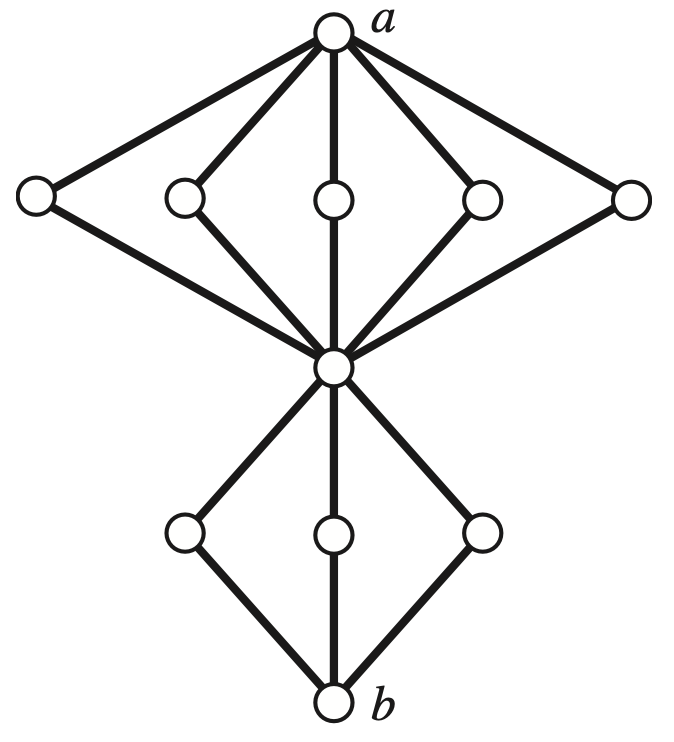
\includegraphics[width=\textwidth]{images/connection_exercise_1} %
    
    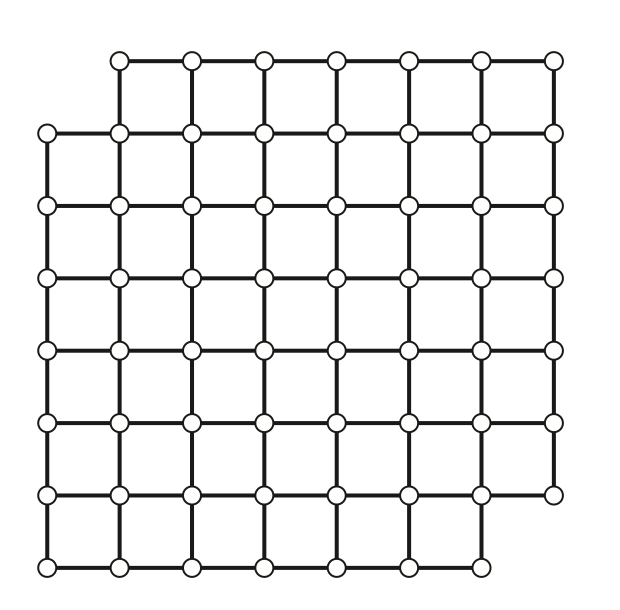
\includegraphics[width=\textwidth]{images/connection_exercise_2}
  
\end{minipage}%    

\end{frame}

\begin{frame}{Solution to group exercise \#1}
\small 
\noindent
\textbf{Problem.} Let $G$ be the graph in the top figure.   (a) How many different paths are there from $a$ to $b$? (b) How many different walks are there from $a$ to $b$?

\begin{center}
    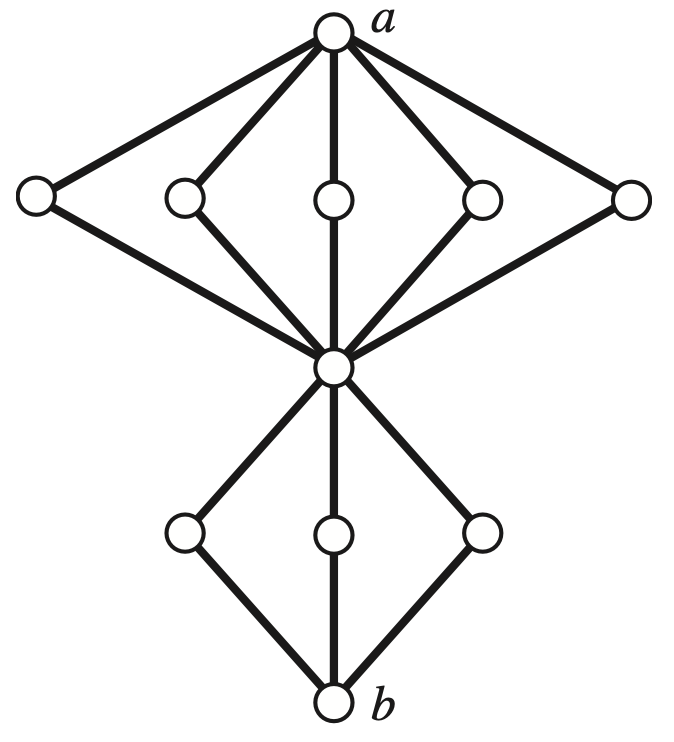
\includegraphics[width=.3\textwidth]{images/connection_exercise_1} %
\end{center}
\vfill 
\textbf{Solution.}
\begin{itemize}
\item[a.] There are 5x3=15 different paths from $a$ to $b$.
\item[b.] There are infinitely many walks from $a$ to $b$.
\end{itemize}

\end{frame}


\begin{frame}{Solution to group exercise \#2}
\small 
\noindent
\textbf{Problem.} Let $G$ be a graph.  A path $P$ in $G$ that contains all the vertices of $G$ is called a \textit{Hamiltonian Path}.  Prove that the graph in the bottom figure of the group exercises does not have a Hamiltonian path.

\vfill 
\textbf{Solution.}  Color the graph as follows.
\begin{center}
    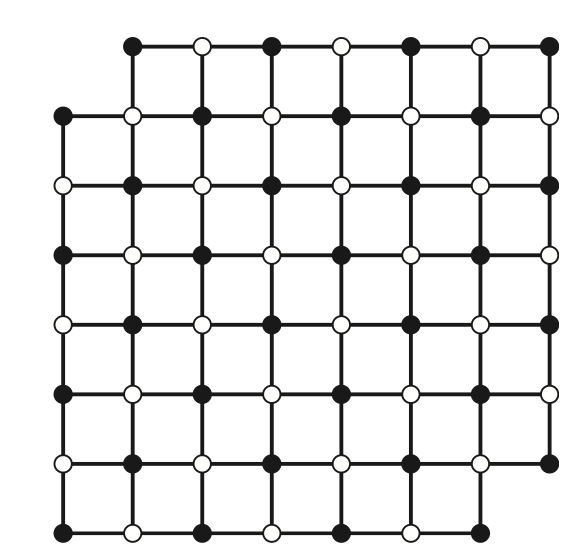
\includegraphics[width=.25\textwidth]{images/connection_hint} %
\end{center}

Suppose a Hamilton path $P$ exists.  We can think of $P$ as list of vertices where each one is adjacent to the next. However, note that neighbors of a white vertex are always black, and neighbors of a black vertex are always white.   Thus $P$ must alternate between black and white vertices.  Now, there are $2(3+5+7)=30$ white vertices and $2(2+4+6) + 8 = 32$ black vertices.  Hence, any enumeration of the 62 vertices must contain at least two consecutive vertices that have the same color. This is a contradiction. 
\end{frame}


\begin{frame}{Solution to group exercise \#3}
\small 
\textbf{Problem.} How many Hamiltonian paths does a complete graph on $n \geq 2$ vertices have?  
\vfill 
\textbf{Solution.} $n!$, since there are $n!$ ways to permute the $n$ vertices. 
\vfill 
\textbf{Remark.} Let's make the argument more concrete.  Let $K_n$ be the complete graph on $n$ vertices.  By enumeration, $K_2$ has two Hamiltonian paths: $a \sim b$ and $b \sim a$. Also by enumeration,  $K_3$ has six Hamiltonian paths: $a \sim b \sim c$, $a \sim c \sim b$,  $b \sim c \sim a$, $b \sim a \sim c$,  $c \sim a \sim b$, and $c \sim b \sim a$. For $K_4$, enumeration is starting to become unwieldy, so we think more abstractly: we have 4 choices for where to start ($a,b,c$ or $d$), then 3 choices of where to go next, then 2 choices for after that, and then the destination spot is determined.

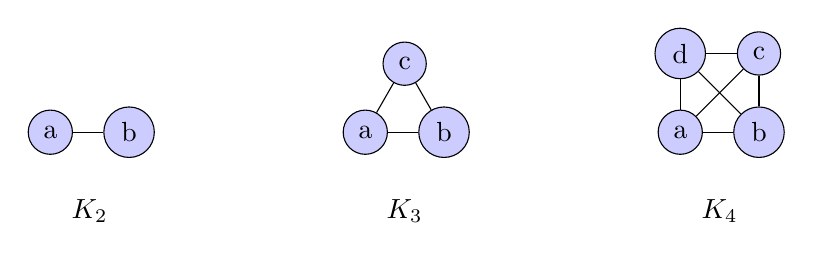
\begin{tikzpicture}[every node/.style={circle, draw, fill=blue!20, minimum size=0.5cm}]
    
    % K2
    \begin{scope}[xshift=0cm]
        \node (a1) at (0,0) {a};
        \node (a2) at (1,0) {b};
        \draw (a1) -- (a2);
		\node[draw=none, fill=none, shape=rectangle] at (0.5,-1) {$K_2$};
    \end{scope}
    
    % K3
    \begin{scope}[xshift=4cm]
        \node (b1) at (0,0) {a};
        \node (b2) at (1,0) {b};
        \node (b3) at (0.5,0.87) {c};
        \draw (b1) -- (b2);
        \draw (b2) -- (b3);
        \draw (b3) -- (b1);
        \node[draw=none, fill=none, shape=rectangle] at (0.5,-1) {$K_3$};
    \end{scope}
    
    % K4
    \begin{scope}[xshift=8cm]
        \node (c1) at (0,0) {a};
        \node (c2) at (1,0) {b};
        \node (c3) at (1,1) {c};
        \node (c4) at (0,1) {d};
        \foreach \i in {1,2,3,4} {
            \foreach \j in {1,2,3,4} {
                \ifnum\i<\j
                    \draw (c\i) -- (c\j);
                \fi
            }
        }
        \node[draw=none, fill=none, shape=rectangle] at (0.5,-1) {$K_4$};
    \end{scope}

\end{tikzpicture}

\end{frame}

\begin{frame}{Solution to group exercise \#4a}
\small 
\textbf{Problem.} Let $G$ be a graph with $n \geq 2$ vertices.   Prove that if G has at least $\binom{n-1}{2} +1$ edges, then $G$ is connected.
\vfill 

\textbf{Solution.}
 We proceed \colorbox{green!30}{by contraposition}.  Suppose $G$ is not connected. Then there is a vertex $v$ not connected to any other vertex.  Thus, there must be at least $n-1$ edges missing from the maximum possible number $\binom{n}{2}$.  That is, there can be no more than $\binom{n}{2} - (n-1)$ edges.  But
    %
    \begin{align*}
    \binom{n}{2} - (n-1) &= 	 \binom{n}{2} -   \binom{n-1}{1} \\
    &= \binom{n-1}{2} && \text{\colorbox{red!30}{\footnotesize{(By Pascal's Identity)}}}
    \end{align*}
    %
    So there are at most $\binom{n-1}{2}$ edges.
\vfill 
\colorbox{green!30}{\textbf{Remark 1.}} Recall that a \colorbox{green!30}{proof by contraposition} proves $A \implies B$ by proving $\lnot B \implies \lnot A$.
\vfill 
\colorbox{red!30}{\textbf{Remark 2.}} From \colorbox{red!30}{Pascal's identity}, we have
\[\binom{n}{2} = \binom{n-1}{1}  + \binom{n-1}{2}  \]
\end{frame}

\begin{frame}{Solution to group exercise \#4b}

\textbf{Problem.} Let $G$ be a graph with $n \geq 2$ vertices.  Show that the result in \#4a is best possible; that is, for each $n \geq 2$, prove there is a graph with 	$\binom{n-1}{2}$ edges that is not connected.
\vfill 

\textbf{Solution.}
    \begin{itemize}
        \item[b.] Select any vertex (we'll call it $v^*$) to isolate.  Of the remaining $n-1$ vertices, form the complete graph $K_{n-1}$.  The subgraph $K_{n-1}$ has $\binom{n-1}{2}$ edges.  However, the full graph $G$ is disconnected, since there is no path that connects $v^*$ to any other vertex.  
    \end{itemize}
\end{frame}



\end{document}
